\documentclass[a4paper,UTF8]{article}
\usepackage{ctex}
\usepackage[margin=1.25in]{geometry}
\usepackage{color}
\usepackage{graphicx}
\usepackage{amssymb}
\usepackage{amsmath}
\usepackage{amsthm}
\usepackage{enumerate}
\usepackage{bm}
\usepackage{hyperref}
\usepackage{epsfig}
\usepackage{color}
\usepackage{mdframed}
\usepackage{lipsum}
\usepackage{mathtools}
\usepackage{hyperref}
\usepackage{diagbox}
\usepackage{float}
\usepackage{caption}
\usepackage{algorithm}
\usepackage{algorithmicx}  
\usepackage{algpseudocode}
\usepackage{amsmath} 
\usepackage{graphicx}
\usepackage{subfigure}
\newmdtheoremenv{thm-box}{myThm}
\newmdtheoremenv{prop-box}{Proposition}
\newmdtheoremenv{def-box}{定义}
\usepackage{listings}
\usepackage{xcolor}
\lstset{
	numbers=left, 
	numberstyle= \tiny, 
	keywordstyle= \color{ blue!70},
	commentstyle= \color{red!50!green!50!blue!50}, 
	frame=shadowbox, % 阴影效果
	rulesepcolor= \color{ red!20!green!20!blue!20} ,
	escapeinside=``, % 英文分号中可写入中文
	xleftmargin=2em,xrightmargin=2em, aboveskip=1em,
	framexleftmargin=2em
} 

\usepackage{booktabs}

\setlength{\evensidemargin}{.25in}
\setlength{\textwidth}{6in}
\setlength{\topmargin}{-0.5in}
\setlength{\topmargin}{-0.5in}

% \setlength{\textheight}{9.5in}
%%%%%%%%%%%%%%%%%%此处用于设置页眉页脚%%%%%%%%%%%%%%%%%%
\usepackage{fancyhdr}                                
\usepackage{lastpage}                                           
\usepackage{layout}                                             
\footskip = 10pt 
\pagestyle{fancy}                    % 设置页眉                 
\lhead{研一下学期}                    
\chead{论文阅读笔记}                                                
% \rhead{第\thepage/\pageref{LastPage}页} 
\rhead{Step2}                                                                                               
\cfoot{\thepage}                                                
\renewcommand{\headrulewidth}{1pt}  			%页眉线宽,设为0可以去页眉线
\setlength{\skip\footins}{0.5cm}    			%脚注与正文的距离           
\renewcommand{\footrulewidth}{0pt}  			%页脚线宽,设为0可以去页脚线

\makeatletter 									%设置双线页眉                                        
\def\headrule{{\if@fancyplain\let\headrulewidth\plainheadrulewidth\fi%
\hrule\@height 1.0pt \@width\headwidth\vskip1pt	%上面线为1pt粗  
\hrule\@height 0.5pt\@width\headwidth  			%下面0.5pt粗            
\vskip-2\headrulewidth\vskip-1pt}      			%两条线的距离1pt        
 \vspace{6mm}}     								%双线与下面正文之间的垂直间距              
\makeatother  

%%%%%%%%%%%%%%%%%%%%%%%%%%%%%%%%%%%%%%%%%%%%%%
\numberwithin{equation}{section}
%\usepackage[thmmarks, amsmath, thref]{ntheorem}
\newtheorem{theorem}{Theorem}
\newtheorem*{definition}{Definition}
\newtheorem*{solution}{Solution}
\newtheorem*{prove}{Proof}
\newcommand{\indep}{\rotatebox[origin=c]{90}{$\models$}}

\usepackage{multirow}

%--

%--
\begin{document}
\title{论文阅读笔记\\
Step2}
\author{MF1833063, 史鹏, spwannasing@gmail.com}
\maketitle
\newpage
\section{Pointer Networks}
我们引入了一种新的神经网络结构来学习输出序列的条件概率,其中的元素是与输入序列中的位置对应的离散序列。这类问题不能通过现在的序列对序列和NTM(Neural Turing Mechines)解决,因为在每个步骤的输出的目标数量取决于输入的长度,这是可变的。诸如排列可变长度序列和各种组合优化问题的问题都属于这个类型。我们的模型采用最近提出的神经注意机制解决了可变大小输出字典的问题。它不同于前面提出的,不是使用注意力机制/将编码器的隐层单元混合在每个解码阶段的上下文向量中,而使用注意力机制作为指针来选择输入序列的一个成员来作为输出序列。我们把这种体系结构叫做指针网络。Ptr-Nets不仅改进了序列到序列(seq-to-seq)的输入注意力机制,而且允许我们将模型泛化去处理可变字典。
\begin{figure}[H]
	\centering
	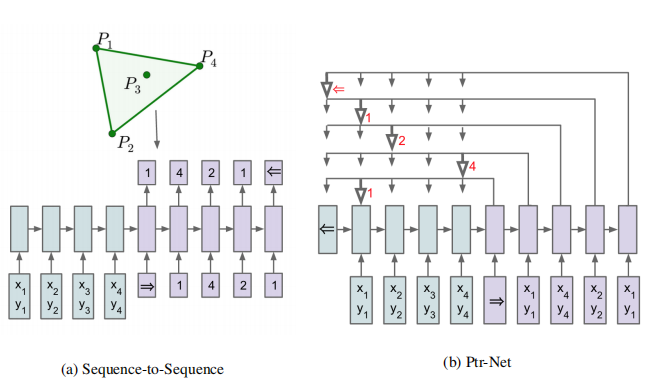
\includegraphics[width=\textwidth]{1-1.png}
	\caption{seq2seq与Prt-Net对比}
\end{figure}
\begin{enumerate}
	\item seq2seq Model\\$$p(C^P|P;\theta)=\prod_{i=1}^{m(P)}p(C_i|C_1,...,C_{i-1},P;\theta)$$
	P是input向量,$C^P$是输出向量,问题就是需要预先设定输出的长度,当输出长度根据输入的不同发生变化的时候就不能很好的完成任务,因为要遍历所有的解空间开销太大了。
	\item Content Based Input Attention\\定义encoder和decoder的hidden state分别为$(e_1,...,e_n)$、$(d_1,...,d_{m(P)})$
	\begin{align*}
		u_j^i&=v^T tanh(W_1e_j+W_2d_i) \\ 
		a_j^i&=softmax(u_j^i) \\ 
		d_i'&=\sum_{j=1}^{n}a_j^ie_j 
	\end{align*}
	然后把$d_i$,$d_i'$连接作为下一个step的隐藏层输入。
	\item Ptr-Net\\
	\begin{align*}
		u_j^i&=v^T tanh(W_1e_j+W_2d_i) \\ 
		p(C_i|C_1,...,C_{i-1},P&=softmax(u_i))
	\end{align*}
	
\end{enumerate}


\newpage
\section{Iterative Alternating Neural Attention for Machine Reading}
和以往的模型不同,不是将query压缩成一个向量,而是部署了部署一种迭代交替的注意机制,允许对查询和文档进行细粒度的探索。
\begin{figure}[H]
	\centering
	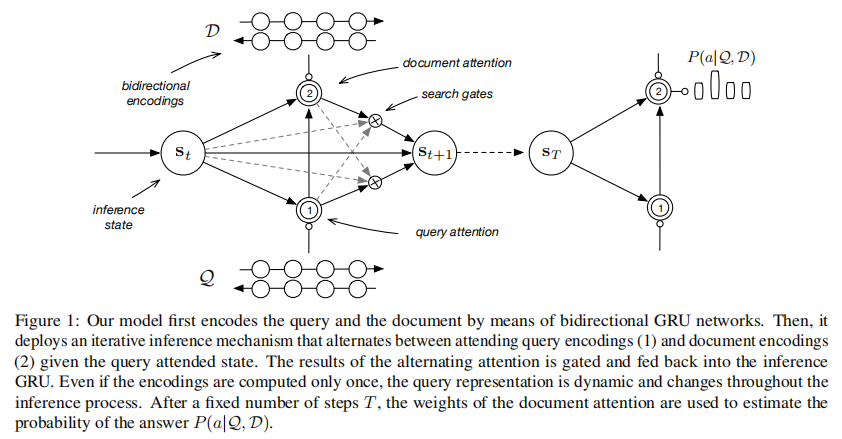
\includegraphics[width=\textwidth]{2-1.png}
	\caption{网络结构图}
\end{figure}
整个推理过程由GRU实现,由以下三部分组成。
\begin{enumerate}
	\item Bidirectional Encoding\\
	将document和query的word embedding送入Bi-RGU,$\widetilde{x}_i=[\overset{\rightarrow}{h_i},\overset{\leftarrow}{h_i}]$
	分别表示为$\widetilde{q}_i \text{,} \widetilde{d}_i$
	\item Iterative Alternating Attention\\
	递归网络迭代地执行交替搜索步骤,以收集可能对预测答案有用的信息。在每一个time step:
	\subitem[1] 对query encoding执行attentive read,得到一个$q_t$
	\subitem[2] 在给定$q_t$的情况下,抽取出$d_t$,代表document中与query相关的部分。\\
	两种抽取都是依据inference GRU $S_{t-1}$之前的隐藏状态:
	\begin{align*}
		q_{i,t}&=\underset{t=1,...,|Q|}{softmax}\tilde{q_i}^T(A_qs_{t-1}+a_q)\\
		q_t &= \sum_i q_{i,t}\tilde{q_i}\\
		d_{i,t}&=\underset{t=1,...,|D|}{softmax}\tilde{d_i}^T(A_d[s_{t-1},q_t]+a_d)\\
		d_t &= \sum_i d_{i,t}\tilde{d_i}
	\end{align*}
	为了更新当前step的hidden state,inference GRU会根据以上两步收集到的信息来进行更新。
	$$ s_t = f([q_t,d_t],s_{t-1})$$
	这里的f是GRU的更新函数。
	\item Answer Prediction\\
	经过固定的时间步之后,根据最后一个step的$d_{i,T}$来预测答案的概率。$$P(a|Q,D)=\sum_{i \in I(a,D)}d_{i,T}$$
	here I(a,D) 是a出现在Document中的位置集合。训练的目标函数就是最大化P。
\end{enumerate}


\newpage
\section{MACHINE COMPREHENSION USING MATCH-LSTM AND ANSWER POINTER}
提出了一种end-to-end的神经网络结构,基于match-LSTM和Pointer Net。又根据Pointer的工作方式分为连续型和boundary型。
\begin{figure}[H]
	\centering
	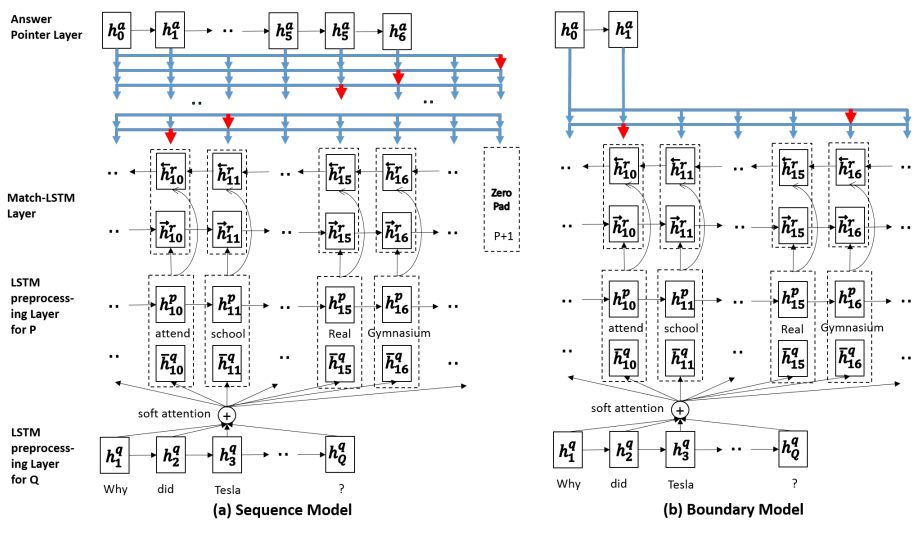
\includegraphics[width=\textwidth]{3-1.png}
	\caption{两种结构对比}
\end{figure}
\begin{enumerate}
	\item Match LSTM\\最初是解决文本蕴含问题提出的,在hypothesis的每一个位置,会通过attention机制来得到一个加权的premise向量。这个向量会被加到这个位置的hypothesis表示中,然后送入LSTM。这个过程叫做match-LSTM。
	\item LSTM Preprocessing Layer$$H^p = \overset{\rightarrow}{LSTM}(P)$$ $$H^q = \overset{\rightarrow}{LSTM}(Q)$$
	\item Match-LSTM Layer\\将query看作premise,passage看作hypothesis。
	\begin{figure}[H]
		\centering
		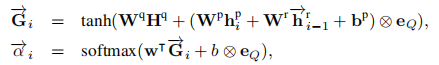
\includegraphics[width=0.6\textwidth]{3-2.png}
	\end{figure}
	$$\overset{\rightarrow}{z}_i = 
	\begin{bmatrix}
		h_i^p\\ 
		H^q\overset{\rightarrow}{\alpha^T}_i
	\end{bmatrix}
	$$
	$$\overset{\rightarrow}{h^r}_i=\overset{\rightarrow}{LSTM}(\overset{\rightarrow}{z}_i,\overset{\rightarrow}{h^{r}}_{i-1})$$
	同时还有另一个反向的LSTM类似以上结构,然后把两个LSTM的输出连接起来。
	$$H^r=\begin{bmatrix}
		\overset{\rightarrow}{H^r}\\
		\overset{\leftarrow}{H^r}
	\end{bmatrix}$$
	\item Answer Pointer Layer\\
	\begin{figure}[H]
		\centering
		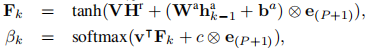
\includegraphics[]{3-3.png}
	\end{figure}
	\begin{figure}[H]
		\centering
		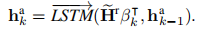
\includegraphics[]{3-4.png}
	\end{figure}
	\begin{figure}[H]
		\centering
		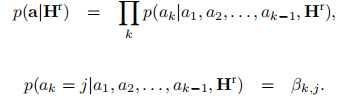
\includegraphics[]{3-5.png}
	\end{figure}
	\begin{figure}[H]
		\centering
		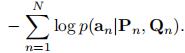
\includegraphics[]{3-6.png}
		\caption{The Sequence Model}
	\end{figure}
	\begin{figure}[H]
		\centering
		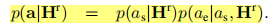
\includegraphics[]{3-7.png}
		\caption{The Boundary Model}
	\end{figure}
\end{enumerate}

\newpage
\section{Gated Self-Matching Networks for Reading Comprehension and Question Answering}
首先通过gated attention-based RNN来得到question-aware的passage表示。然后提出了使用self-matching来获得更加细粒度的表示。
\begin{figure}[H]
	\centering
	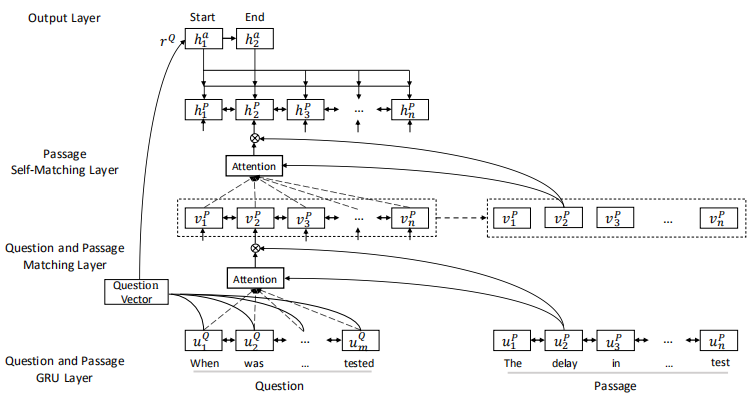
\includegraphics[width=\textwidth]{4-1.png}
	\caption{结构图}
\end{figure}
\begin{enumerate}
	\item Question and Passage Encoder\\使用了word-level和character-lever的embedding,然后送入BiRNN
	\begin{align*}
		u_t^Q&=BiRNN_Q(u_{t-1}^Q,[e_t^Q,c_t^Q])\\
		u_t^P&=BiRNN_P(u_{t-1}^P,[e_t^P,c_t^P])
	\end{align*}
	\item Gated Attention-based Recurrent Networks\\
	sentence-pair representation :
	$$v_t^P=RNN(v_{t-1}^P,c_t)$$here $c_t = att(c^Q,[u_t^P,v_{t-1}^P])$
	\begin{align*}
		s_j^t&=v^Ttanh(W_u^Qu_j^Q+W_u^Pu_t^P+W_v^Pv^P_{t-1})\\
		a_i^t&=\frac{s_i^t}{\sum_{j=1}^{m}s_j^t}\\
		c_t&=\sum_{i=1}^{m}a_i^tu_i^Q
	\end{align*}
	match-LSTM:\\$$v_t^P = RNN(v_{t-1}^P,[u_t^P,c_t])$$
	add another gate:\\
	\begin{align*}
		g_t&=sigmoid(W_g[u_t^P,c_t])\\
		[u_t^P,c_t]^*&=g_t\odot[u_t^P,c_t]
	\end{align*}
	然后就用这个代替原本的$[u_t^P,c_t]$,这就是gated attention-based Recurrent Network。这个gate有效的建模了只有passage中的部分与问题相关的这个现象。
	\item Self-Matching Attention\\
	$$h_t^P=RNN(h_{t-1}^P,[v_t^P,c_t])$$here $c_t = att(v^P,v_t^P)$
	\begin{align*}
		s_j^t&=v^Ttanh(W_v^Pv_j^P+W_v^{\tilde{P}}v_t^P)\\
		a_i^t&=\frac{s_i^t}{\sum_{j=1}^{n}s_j^t}\\
		c_t&=\sum_{i=1}^{m}a_i^tv_i^P
	\end{align*}
	这里也使用了同上的additional gate。
	\item Output Layer\\
	\begin{figure}[H]
		\centering
		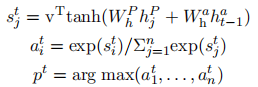
\includegraphics[]{4-2.png}
	\end{figure}
	\begin{figure}[H]
		\centering
		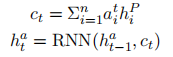
\includegraphics[]{4-3.png}
	\end{figure}
	\begin{figure}[H]
		\centering
		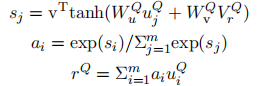
\includegraphics[]{4-4.png}
	\end{figure}
	
\end{enumerate}
\newpage
\section{Attention-over-Attention Neural Networks for Reading Comprehension}
提出了一种简单但是有效的模型,在document-level Attention上又放置了一层Attention。另外一个贡献是提出了N-best-reranking策略。
\begin{figure}[H]
	\centering
	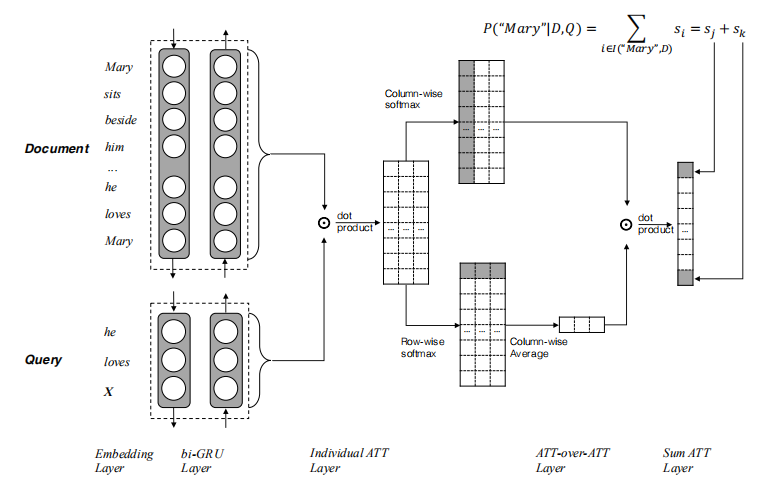
\includegraphics[width=\textwidth]{5-1.png}
	\caption{网络结构图}
\end{figure}
\begin{enumerate}
	\item Attention-over-Attention\\
	$$M(i,j)=h_{doc}(i)^T\dot h_{query}(j)$$
	然后分别对行和列进行softmax运算。
	$$ \alpha(t)= softmax(M(1, t), ..., M(|D|, t)) $$
	$$ \alpha =[\alpha(1),...,\alpha(|Q|)]$$
	$$\beta(t) = sof tmax(M(t, 1), ..., M(t, |Q|))$$
	$$\beta = \frac{1}{n}\sum_{t=1}{|D|}\beta(t)$$
	$$s=\alpha^T\beta$$
	$$P(w|D, Q) = \sum_{i \in I(w,D)}s_i$$
	训练目标:最大化:$\mathcal{L}=\sum_i log(p(x)),x\in \mathcal{A}$
	\item N-best-Reranking\\
	不是选出分数最高的作为答案,而是在解码的过程中生成最好的N个候选答案列表。将N个候选答案填入句子,用语言模型来对句子进行打分,重新选出得分最高的答案。
\end{enumerate}


\newpage
\section{BI-DIRECTIONAL ATTENTION FLOW FOR MACHINE COMPREHENSION}
\begin{figure}[H]
	\centering
	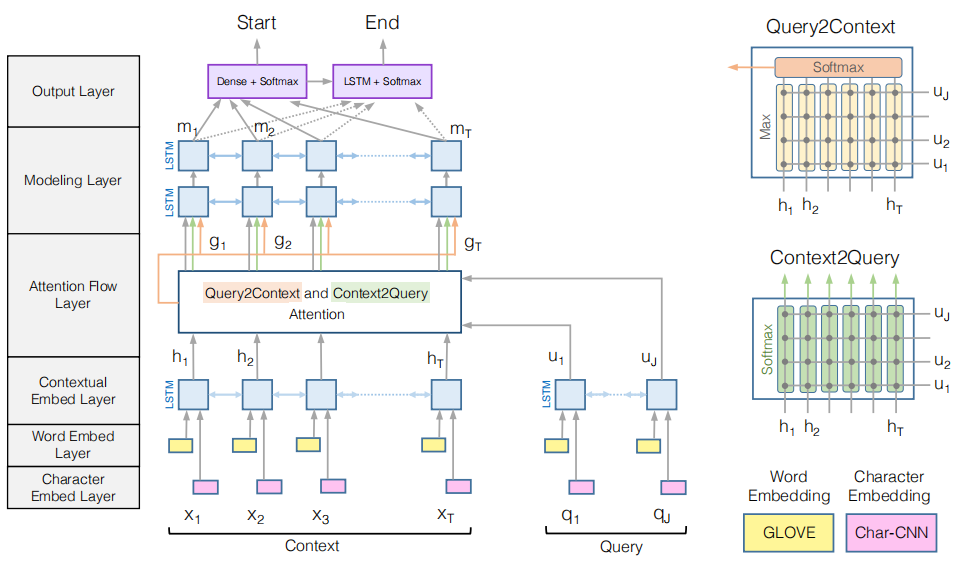
\includegraphics[width=\textwidth]{6-1.png}
	\caption{BiDirectional Attention Flow Model}
\end{figure}
\begin{enumerate}
	\item Attention Flow Layer\\H和U分别为经过BiLSTM的context和query。$S\in \mathbb{R}^{T \times J}$计算H和U的相似度。
	$$S_{tj}=\alpha(H_{:t},U_{:j})$$这里选择$\alpha(h,u)=w^T_{(S)}[h;u;h\circ u]$
	\subitem[1] Context-to-query Attention$$a_t=softmax(S_{t:})$$ $$\tilde{U_{:t}}=\sum_j a_{tj}U_{:j}$$
	\subitem[2] Query-to-context Attention\\$$b = softmax(max_{col}(S))$$ $$\tilde{h} =\sum_t b_tH_{:t}$$
	将其在列方向重复T遍组成$\tilde{H}$。
	$$G_{:t}=\beta(H_{:t},\tilde{U_{:t}},\tilde{H_{:t}})$$
	\item Modeling Layer\\将G送入LSTM,得到矩阵$M\in \mathbb{R}^{2d\times T}$
	\item Output Layer$$p^1=softmax(w_{p^1}^T[G,M])$$
	将M送入另一个Bi-LSTM,得到$M^2$ $$p^2=softmax(w_{p^2}^T[G,M^2])$$
	\item Training$$L(\theta)=-\frac{1}{N}\sum_{i}^{N}log(p_{y_i^1}^1)+log(p_{y_i^2}^2)$$
\end{enumerate}
\newpage
\section{Gated-Attention Readers for Text Comprehension}
提出了一种multi-hop结构,结合一种新的注意力机制。在GA Reader的迭代中,逐渐细化embedding的上下文表示。
\begin{figure}[H]
	\centering
	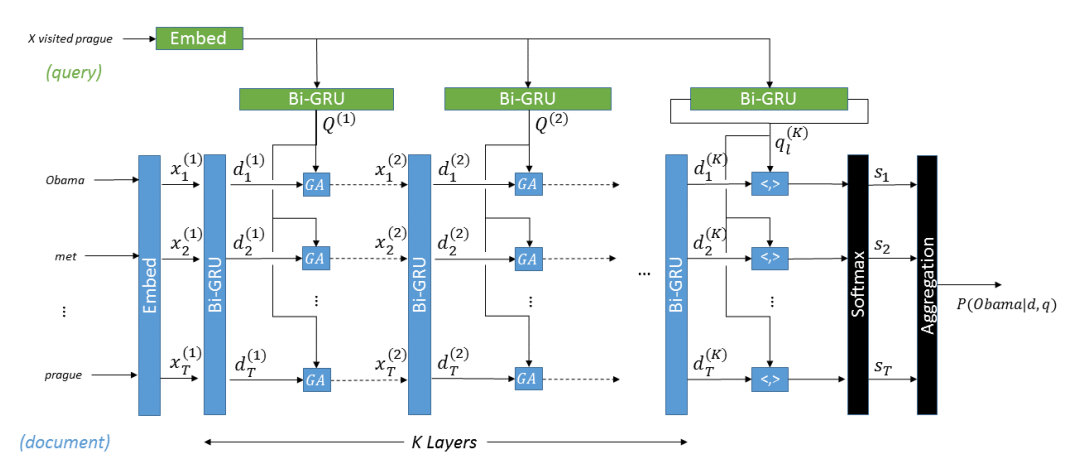
\includegraphics[width=\textwidth]{7-1.png}
	\caption{网络结构}
\end{figure}
\begin{enumerate}
	\item Multi-Hop Architecture\\$$D^{(k)}=\overset{\leftrightarrow }{GRU}_D^{(k)}(X^{(k-1)})$$
	$$Q^{(k)}=\overset{\leftrightarrow}{GRU}_Q^{(k)}(Y)$$
	$$X^{(k)}=GA(D^{(k)},Q^{(k)})$$
	\item Gated-Attention Module\\
	\begin{align*}
		\alpha_i&=softmax(Q^Td_i)\\
		\tilde{q}_i&=Q\alpha_i\\
		x_i&=d\odot \tilde{q}_i
	\end{align*}
	\item Answer Prediction\\$$s=softmax((q_l^{(K)})^TD^{(K)})$$
	$$Pr(c|d,q) \propto \sum s_i$$
\end{enumerate}
\newpage
\section{A Constituent-Centric Neural Architecture for Reading Comprehension}
提出了一种Tree LSTM以及Chain-of-trees LSTM。将解析树与LSTM相结合。
\begin{figure}[H]
	\centering
	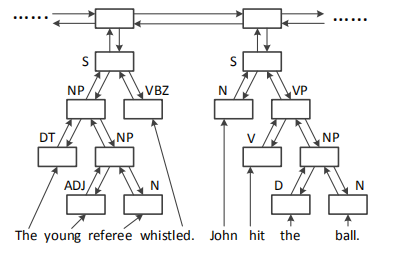
\includegraphics[]{8-1.png}
	\caption{Chain-of-trees LSTM}
\end{figure}
\begin{figure}[H]
	\centering
	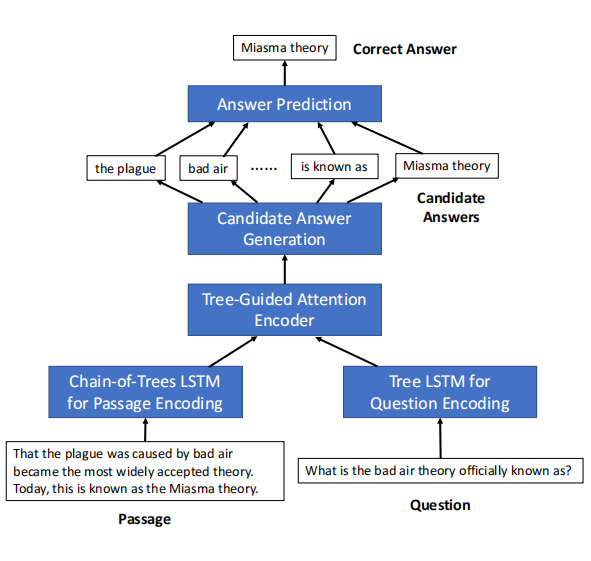
\includegraphics[width=0.7\textwidth]{8-2.png}
	\caption{Constituent-centric neural network}
\end{figure} 


\newpage
\section{Structural Embedding of Syntactic Trees for Machine Comprehension}
提出了SEST以及SEDT,利用句子的结构信息并将其embedding。
\begin{figure}[H]
	\centering
	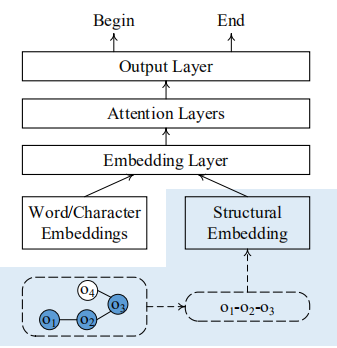
\includegraphics[]{9-1.png}
\end{figure}
\begin{figure}[H]
	\centering
	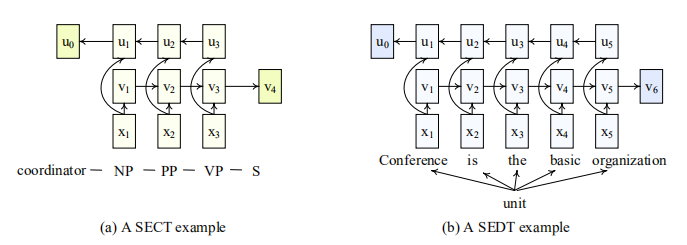
\includegraphics[width=\textwidth]{9-2.png}
\end{figure}

\newpage
\section{Accurate Supervised and Semi-Supervised Machine Reading for Long}
将文档切分为一个个小的,重叠的window,然后通过RNN来并行的编码。提出了Sliding-Window Encoder Attentive Reader(SWEAR)模型。另外还提出了一个半监督学习的版本。
\begin{figure}[H]
	\centering
	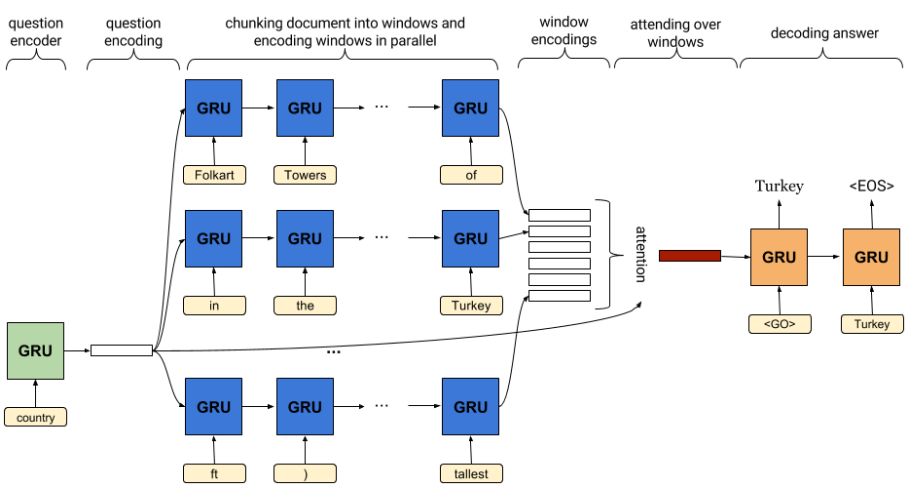
\includegraphics[width=\textwidth]{10-1.png}
\end{figure}
\end{document}